\begin{mainquestion}{parallelrlc}{Parallel RLC Impedance}

Consider the current-driven parallel $RLC$ circuit shown to the right.

\begin{center}
    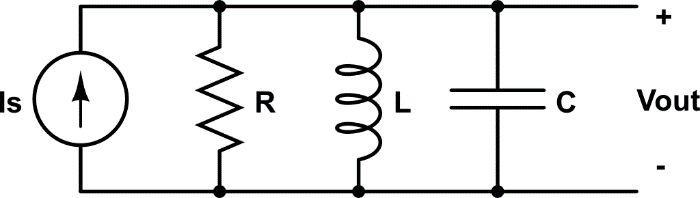
\includegraphics[width=4.7in]{circuit.png}
\end{center}

\begin{partquestion}{deriveimpedance}{Derive the impedance $Z\left(j\omega\right)$ facing the current source. Express your answer explicitly as the sum of the real and imaginary part.}
\begin{answer}
The total impedance facing the current source will be the parallel combination of the individual impedances, as shown below:

\[
Z\left(j\omega\right) = Z_{R} \parallel Z_{L} \parallel Z_{C} = \frac{1}{\frac{1}{Z_{R}} + \frac{1}{Z_{L}} + \frac{1}{Z_{C}}} = \frac{1}{\frac{1}{R} + \frac{1}{j\omega L} + j\omega C} = \frac{1}{\frac{1}{R} + j\left(\omega C - \frac{1}{\omega L}\right)}
\]

We then simplify by multiplying both the numerator and denominator by the complex conjugate of the denominator, as shown below:
\begin{align*}
Z\left(j\omega\right) &= \frac{1}{\frac{1}{R}+j\left(\omega C-\frac{1}{\omega L}\right)}\cdot\frac{\frac{1}{R}-j\left(\omega C-\frac{1}{\omega L}\right)}{\frac{1}{R}-j\left(\omega C-\frac{1}{\omega L}\right)}\\
&=\frac{\frac{1}{R}-j\left(\omega C-\frac{1}{\omega L}\right)}{\frac{1}{R^2}+\left(\omega C-\frac{1}{\omega L}\right)^2}\\
&=\frac{\frac{1}{R}}{\frac{1}{R^2}+\left(\omega C-\frac{1}{\omega L}\right)^2}-j\frac{\left(\omega C-\frac{1}{\omega L}\right)}{\frac{1}{R^2}+\left(\omega C-\frac{1}{\omega L}\right)^2}
\end{align*}
\end{answer}
\end{partquestion}

\begin{partquestion}{maxmagnitude}{At what frequency is the magnitude of the impedance $\left|Z\left(j\omega\right)\right|$ a maximum? What is the phase angle at that frequency?}
\begin{answer}
We find $\left| Z(j\omega) \right|$ as shown below:

\begin{align*}
\left|Z\left(j\omega\right)\right| &= \left|\frac{\frac{1}{R}-j\left(\omega C-\frac{1}{\omega L}\right)}{\frac{1}{R^2}+\left(\omega C-\frac{1}{\omega L}\right)^2}\right|\\
&=\frac{1}{\sqrt{\frac{1}{R^2}+\left(\omega C-\frac{1}{\omega L}\right)^2}}
\end{align*}

We note that maximizing $\left| Z(j\omega) \right|$ is equivalent to minimizing its denominator. By inspection, we can see that the denominator is minimized when $\omega C = \frac{1}{\omega L}$, which occurs at:

\[
\omega_{0} = \frac{1}{\sqrt{LC}}
\]

In other words, this maximum occurs when the capacitive impedance is equal to the inductive impedance, and the total impedance is just $Z\left(j\omega_{0}\right) = R$. From our first equation in part (\cref{prob:parallelrlc:deriveimpedance}), we can find the phase angle:

\begin{align*}
\angle Z\left(j\omega\right) &= \angle \frac{1}{\frac{1}{R}+j\left(\omega C-\frac{1}{\omega L}\right)}\\
&=\angle 1-\angle\left(\frac{1}{R}+j\left(\omega C-\frac{1}{\omega L}\right)\right)\\
&=0-\tan^{-1}\left[\frac{\omega C-\frac{1}{\omega L}}{\frac{1}{R}}\right]\\
&=-\tan^{-1}\left[\omega RC-\frac{R}{\omega L}\right]
\end{align*}

And it follows that at $\omega = \omega_{0} = \frac{1}{\sqrt{LC}}$, we have:

\begin{align*}
\angle Z\left(j\omega_0\right) &= -\tan^{-1}\left[\omega_0 RC-\frac{R}{\omega_0 L}\right]\\
&= -\tan^{-1}\left[\frac{RC}{\sqrt{LC}}-\frac{R\sqrt{LC}}{L}\right]\\
&= -\tan^{-1}\left[\frac{R\sqrt{C}}{\sqrt{L}}-\frac{R\sqrt{C}}{\sqrt{L}}\right]\\
&= -\tan^{-1}0\\
&= 0
\end{align*}

We could also have easily arrived at this answer by noting (see above) that at $\omega_{0}$ the total impedance becomes $Z = R$, which has a phase of 0 because $R$ is just a real number.
\end{answer}
\end{partquestion}

\begin{partquestion}{extremephase}{What is the phase angle of the impedance at zero (DC) and at extremely high frequency? Provide an intuitive explanation based on the behavior of $C$ and $L$ in these extremes.}
\begin{answer}
At very low frequencies (DC), the inductor behaves like a short circuit, which offers the least impedance path for the incoming current $I_{S}$. It is important to note that the resistor still remains a resistor and the capacitor behaves like an open circuit. The effect of this asymptotic behavior is that the impedance, $Z(j\omega) = R \parallel j\omega L \parallel \frac{1}{j\omega C} \approx j\omega L$ is dominated by the inductor (because $j\omega L$ becomes very small). Since $Z(j\omega) \approx j\omega L = \omega Le^{j\frac{\pi}{2}}$, we should observe the phase angle approaches $\lim\limits_{\omega\to0^+}\angle Z(j\omega)=\frac{\pi}{2}=+90^\circ$.

At extremely high frequency, the capacitor behaves like a short, the inductor like an open, and the resistor remains a resistor. Thus, $Z(j\omega) = R \parallel j\omega L \parallel \frac{1}{j\omega C} \approx \frac{1}{j\omega C}$ is dominated by the capacitor (because $j\omega C$ becomes very large). As such, $Z(j\omega) \approx \frac{1}{j\omega C} = \frac{-j}{\omega C} = \frac{1}{\omega C}e^{-j\frac{\pi}{2}}$ and we observe that the phase angle approaches $\lim\limits_{\omega\to\infty}\angle Z(j\omega)=-\frac{\pi}{2}=-90^\circ$.
\end{answer}
\end{partquestion}

\begin{partquestion}{bodeplots}{Let $R = 7\text{ k}\Omega$, $L = 1\text{ mH}$, and $C = 1\text{ nF}$. Create Bode plots for both the magnitude and phase of the transfer function $\frac{V_{\text{out}}}{I_{S}}$. Note that this transfer function is the impedance of the network, so you do not need to re-derive it!}
\begin{answer}
We can use our first equation from part (\cref{prob:parallelrlc:deriveimpedance}) and massage it into a form that MATLAB will like:

\[
Z\left(j\omega\right) = \frac{1}{\frac{1}{R} + \frac{1}{j\omega L} + j\omega C} = \frac{j\omega L}{\left(j\omega \right)^2LC+\frac{j\omega L}{R} + 1}
\]

Using the following simple MATLAB script:

\begin{verbatim}
L=1e-3;
R=7e3;
C=1e-9;
num=[L 0];
den=[C*L L/R 1];
bode(num,den);
\end{verbatim}

We can generate the Bode plots for magnitude and phase of $Z\left(j\omega\right)$:

\begin{center}
    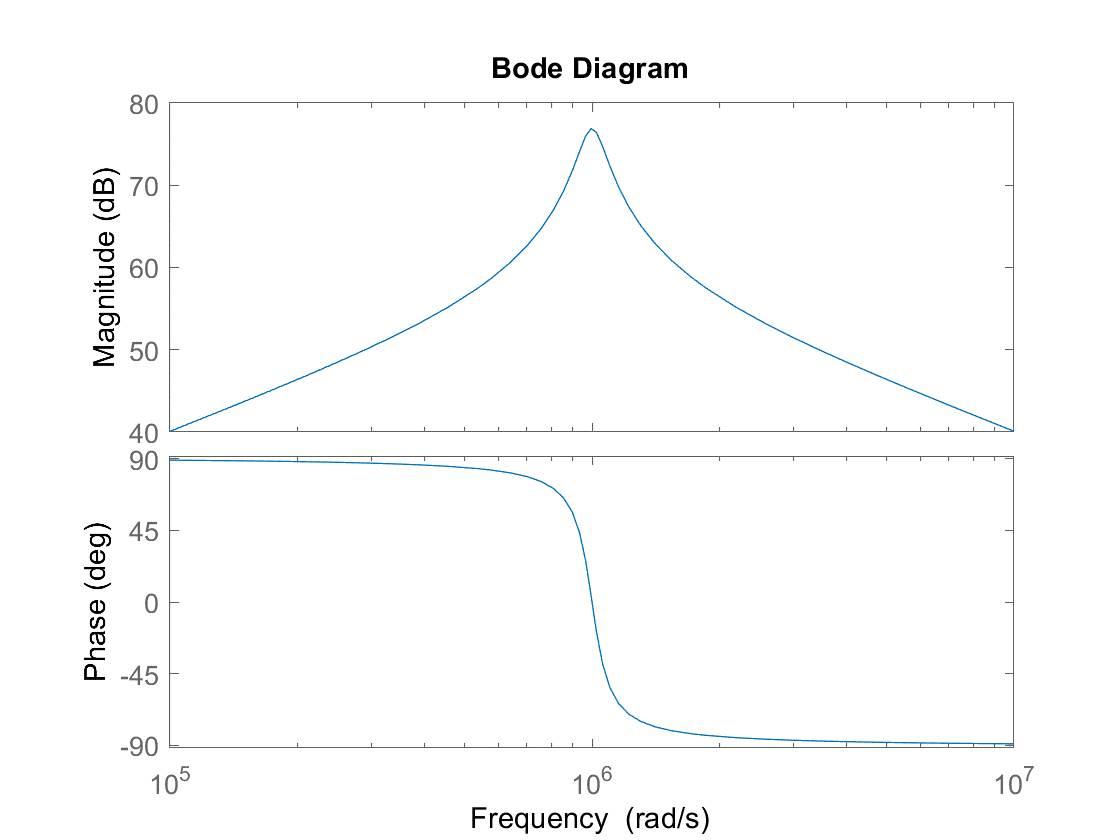
\includegraphics[width=5.25in]{bode_plot.png}
\end{center}
\end{answer}
\end{partquestion}

\end{mainquestion}